\chapter{Εισαγωγή}
\label{ch:chapter1}

Η ανάπτυξη των Μεγάλων Γλωσσικών Μοντέλων \textlatin{(LLM)} έχει
επιφέρει ριζικές αλλαγές στον τομέα της Τεχνητής Νοημοσύνης και της
Επεξεργασίας Φυσικής Γλώσσας \textlatin{(NLP)} \cite{bommasani2021opportunities,zhao2023survey,zhou2023comprehensive,jurafsky2009speech}.
Η εισαγωγή αυτών των μοντέλων στην καθημερινή ζωή μέσω του
\textlatin{Chat-GPT} το 2022 \cite{openai2022chatgpt} έχει πυροδοτήσει
μια επανάσταση στην τεχνολογική αγορά, σηματοδοτώντας την απαρχή του
αγώνα για την κυριαρχία στην αγορά της Τεχνητής Νοημοσύνης \cite{guardian2024openai,nyt2024openai,verge2023chatgpt,liu2023chatgpt,trendforce2023ai}.
Τα μοντέλα αυτά έχουν αποδειχθεί εξαιρετικά αποτελεσματικά στην
αντιμετώπιση προβλημάτων επεξεργασίας φυσικής γλώσσας, όπως η αναγνώριση
φυσικής γλώσσας, προάγοντας την ανάπτυξη της Γενικής Τεχνητής Νοημοσύνης
\textlatin{(AGI)} \cite{adams2012mapping,goertzel2014agi}.

Μέσα σε αυτή την επανάσταση, η χρήση μοντέλων επεξεργασίας φυσικής
γλώσσας στον τομέα του προγραμματισμού και της ανάπτυξης λογισμικού,
ονόματι βοηθοί κώδικα \textlatin{(Code Assistants)}, έχει αναδειχθεί ως
ένας από τους πιο υποσχόμενους τομείς της τεχνολογίας. Ένα από τα πιο
διαδεδομένα εργαλεία με αυτόν το σκοπό είναι το \textlatin{GitHub
  Copilot} \cite{github2021copilot,githubcopilot}. Αναπτυγμένο σε
συνεργασία με την \textlatin{OpenAI}, το \textlatin{GitHub Copilot}
ξεκίνησε χρησιμοποιώντας το μοντέλο ονόματι \textlatin{Codex} της
\textlatin{OpenAI} \cite{chen2021evaluating}, σχεδιασμένο εξ' αρχής
αποκλειστικά για τη παραγωγή κώδικα, για να προτείνει κώδικα στον
προγραμματιστή κατά την γραφή κώδικα.

Η παροδική απόσυρση του μοντέλου \textlatin{Codex} τον Μάρτιο του 2023
και η οριστική του απόσυρση το 2023 \cite{kemper2023openai}, οδήγησε
στην ανάπτυξη ενός νέου μοντέλου, σε συνεργασία μεταξύ της
\textlatin{OpenAI}, της \textlatin{Microsoft Azure AI}, και της
\textlatin{GitHub AI}. Το νέο μοντέλο αρχικά βασίστηκε στο
\textlatin{GPT-3.5 Turbo} \cite{github2023copilotupdate}, με την επόμενή
του έκδοση να βασίζεται στο \textlatin{GPT-4}
\cite{github2023copilotupdate}, με το κωδικό όνομα \textlatin{GitHub
  Copilot X} \cite{github2023copilotx}, δίνοντας την δυνατότητα για μια
νέα λειτουργία, του \textlatin{GitHub Copilot Chat}, ενός
\textlatin{chatbot} μοντέλου, παρόμοιο με αυτό του \textlatin{Chat-GPT}.
Μέσω αυτής της λειτουργίας, ο προγραμματιστής μπορεί μέσα από το
περιβάλλον ανάπτυξής του \textlatin{(IDE)}, να κάνει ερωτήσεις στο
μοντέλο, χρησιμοποιώντας φυσική γλώσσα, ενώ το μοντέλο μπορεί να
χρησιμοποιήσει τον ήδη υπάρχοντα κώδικα, την τεκμηρίωση, και τις οδηγίες
του προγραμματιστή για να απαντήσει στην ερώτηση του προγραμματιστή.

\begin{figure}[H]
  \begin{center}
    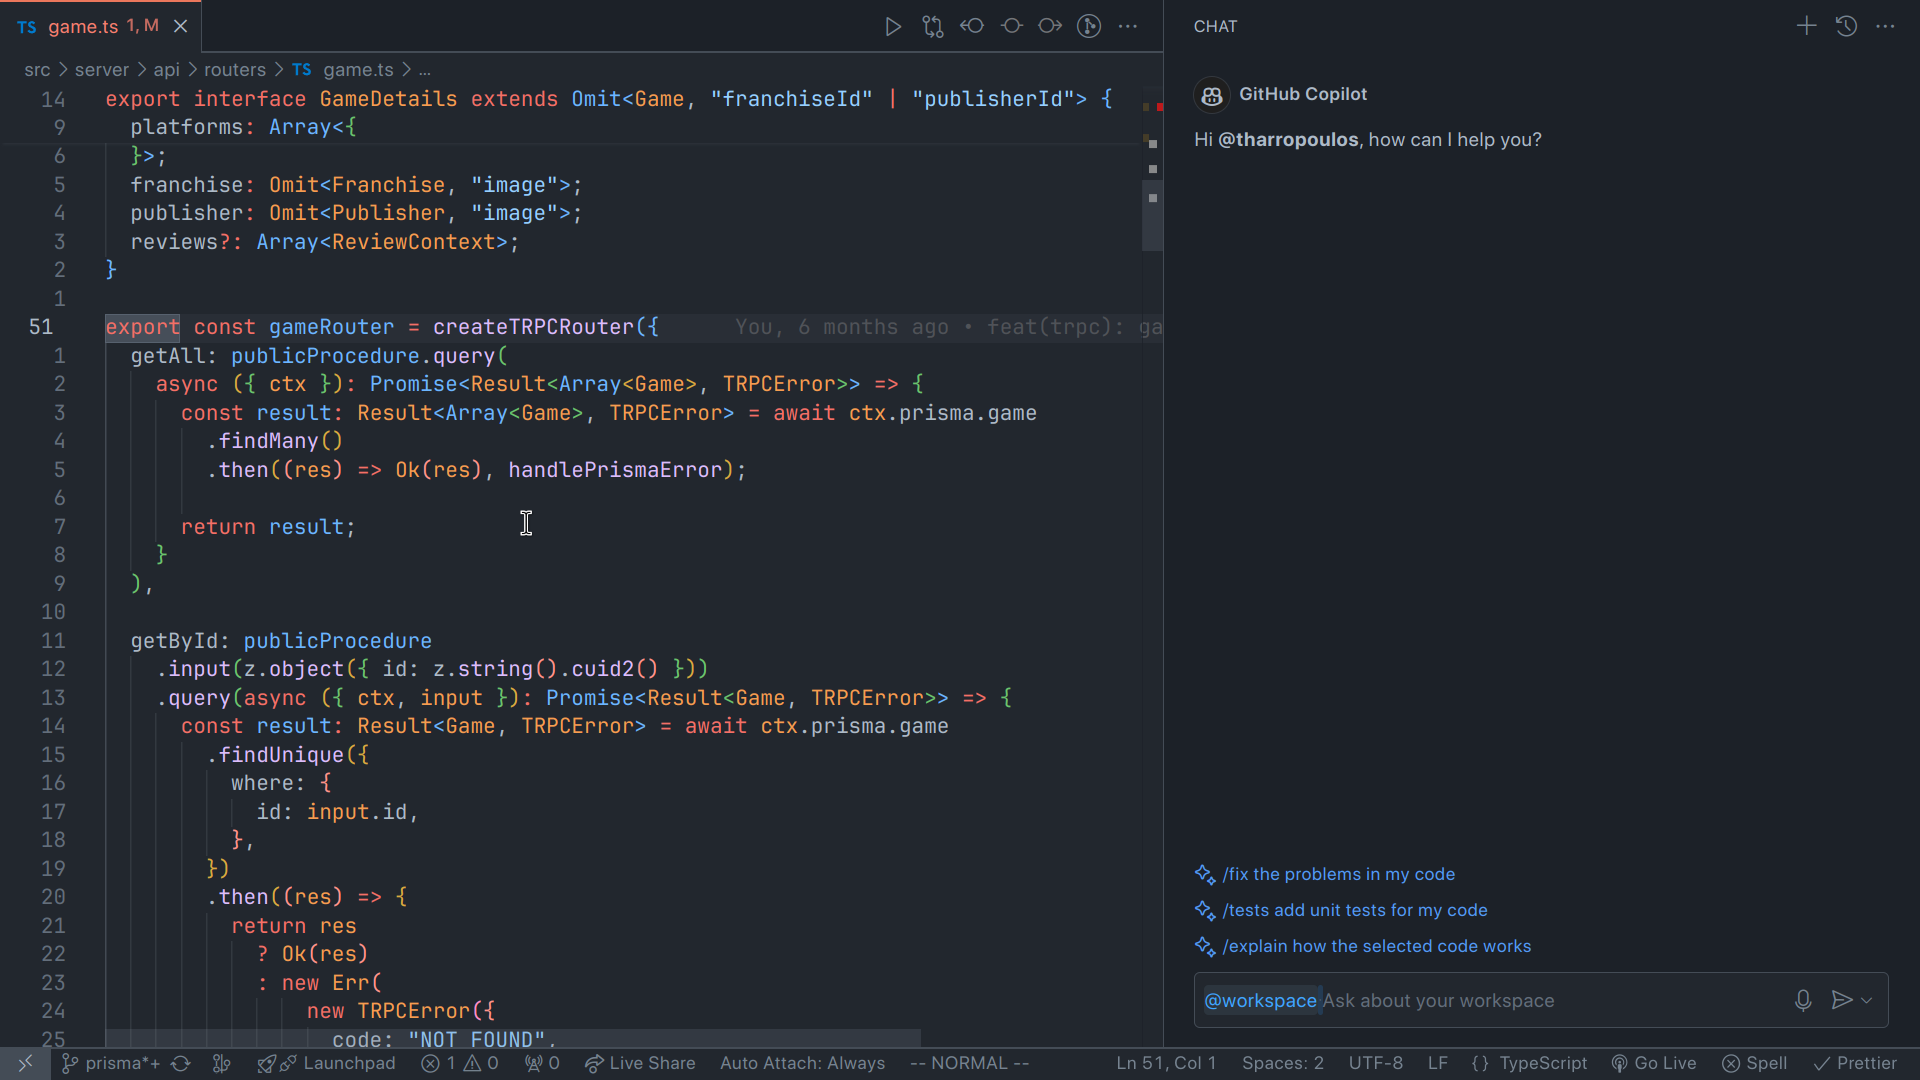
\includegraphics[width=\textwidth]{copilotchat screen.png}
    \label{fig:codeComp}
    \caption{Παράδειγμα χρήσης του \textlatin{GitHub Copilot Chat} εντός
      του \textlatin{IDE} \textlatin{Visual Studio Code}
      \cite{vscodeintro, vscode} }
  \end{center}
\end{figure}

Το \textlatin{GitHub Copilot Chat} αρχικά ήταν διαθέσιμο μόνο μέσω
λίστας αναμονής, με την πρόσβαση να δίνεται σε περιορισμένο αριθμό
προγραμματιστών, κατόπιν αίτησης, με την ενσωμάτωση του
\textlatin{GPT-4} να γίνεται επίσημα τον Νοέμβριο του 2023
\cite{github2023gpt4}. Η δημόσια κυκλοφορία του \textlatin{GitHub
  Copilot Chat} έγινε τον Δεκέμβριο του 2023 \cite{github2023chat}.

Πέρα από το \textlatin{GitHub Copilot}, υπάρχουν πολλοί άλλοι
\textlatin{code assistants}, με αυτούς που λήφθηκαν υπ' όψιν να είναι
οι:
\begin{itemize}
\item
  \textlatin{Tabnine} \cite{microsoft2021tabnine, vincent2019ai}
\item
  \textlatin{Codeium} \cite{forbes2024codeium}
\item
  \textlatin{Amazon Codewhisperer} \cite{bays2022AWS}
\end{itemize}
Η απόφαση για την χρήση του \textlatin{GitHub Copilot} ως το εργαλείο,
του οποίου η λειτουργία θα εξεταστεί στην παρούσα διπλωματική, έγινε με
βάση την ευρεία χρήση του, την ενσωμάτωση του μοντέλου
\textlatin{GPT-4}, και την δυνατότητα χρήσης του \textlatin{GitHub
  Copilot Chat}, καθώς και την δωρεάν παροχή του σε ενεργούς φοιτητές
του Αριστοτελείου Πανεπιστήμιου Θεσσαλονίκης μέσω του προγράμματος
\textlatin{GitHub Student Developer Pack} \cite{githubstudentpack}.

\section{Δημιουργία Κώδικα \textlatin{(Code Generation)} - Ολοκλήρωση
  Κώδικα \textlatin{(Code Completion)} }

\label{sec:ch1-}

Δύο όροι που συχνά συναντώνται στην βιβλιογραφία είναι η
\textbf{Δημιουργία Κώδικα} \textlatin{(Code Generation)} και η
\textbf{Ολοκλήρωση Κώδικα} \textlatin{(Code Completion)}. Και οι δύο
όροι έχουν άμεση σχέση με την παραγωγικότητα του προγραμματιστή και
αποτελούν σημαντικά εργαλεία για την ανάπτυξη λογισμικού \cite{codecomp,
  koester1996effect, asaduzzaman2014cscc}, και ενώ και τα δύο μπορούν να
χρησιμοποιήσουν μοντέλα Τεχνητής Νοημοσύνης
\cite{svyatkovskoy2020fast,raychev2014code} με την διαφορά να βρίσκεται
στον τρόπο λειτουργίας τους.

\subsection*{Ολοκλήρωση Κώδικα} Σύμφωνα με
\textlatin{\citeauthor{Omar2012}} \cite{Omar2012}, η Ολοκλήρωση Κώδικα
αφορά εργαλεία που τα περισσότερα περιβάλλοντα ανάπτυξης παρέχουν μέσω
της μορφής πλωτού μενού που περιέχει συμφραζόμενες-σχετικές μεταβλητές,
πεδία, μεθόδους, τύπους και άλλα αποσπάσματα κώδικα. Επιλέγοντας από
αυτό το μενού, οι προγραμματιστές μπορούν να αποφύγουν πολλά συνηθισμένα
ορθογραφικά και λογικά λάθη και να εξαλείψουν τις περιττές
πληκτρολογήσεις. Το βασικό εργαλείο που χρησιμοποιείται για την επίτευξη
του σκοπού αυτού είναι το \textlatin{Language Server Protocol (LSP)} της
\textlatin{Microsoft}, δίνοντας την δυνατότητα σε κάθε περιβάλλον
ανάπτυξης να επικοινωνήσει με την εξωτερική διεργασία του
\textlatin{Language Server} και να λάβει πληροφορίες για τον κώδικα που
γράφεται, όπως τις προτάσεις ολοκλήρωσης κώδικα, τα λάθη, και τις
προτάσεις διόρθωσης, σε μια διάταξη χρήστη - διακομιστή \cite{Rask2022,
  Bunder2019}.

\begin{figure}[H]
  \begin{center}
    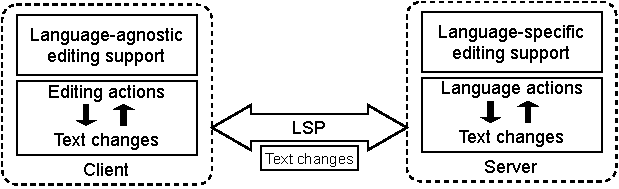
\includegraphics{LSPApproach.pdf}
    \label{fig:LSP_architecture}
    \caption{Η αρχιτεκτονική του \textlatin{Language Server Protocol},
      \textit{Δανεισμένο από \cite{Rodriguez-Echeverria2018}}}
  \end{center}
\end{figure}

Η Ολοκλήρωση Κώδικα δεν παράγει κώδικα από το μηδέν, αλλά προτείνει
συμπληρωματικές λύσεις στον υπάρχοντα κώδικα, βοηθώντας τον
προγραμματιστή να ολοκληρώσει τον κώδικα του ταχύτερα.

\begin{figure}[H]
  \begin{center}
    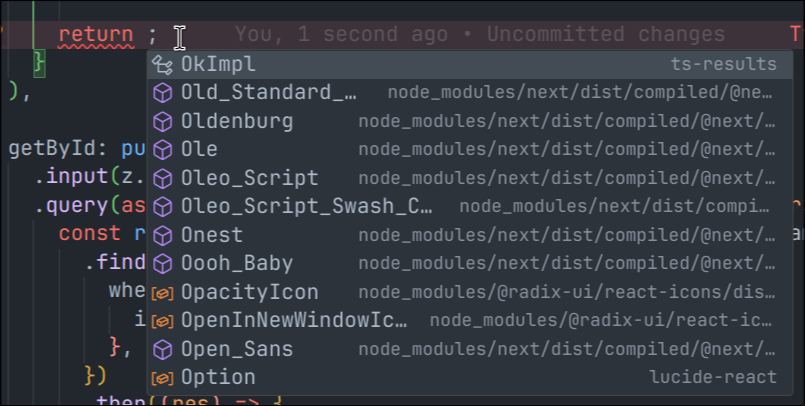
\includegraphics[width=\textwidth]{codeComp.png}
    \label{fig:codeComp}
    \caption{Παράδειγμα Ολοκλήρωσης Κώδικα εντός του \textlatin{IDE}
      \textlatin{Visual Studio Code} }
  \end{center}
\end{figure}

\subsection*{Δημιουργία Κώδικα} Η Δημιουργία Κώδικα αφορά την άμεση
παραγωγή κώδικα από ένα μοντέλο στοχασχτικά, με βάση το συγκείμενο
κώδικα του προγραμματιστή. To μοντέλο που χρησιμοποιείται για την
παραγωγή κώδικα είναι εκπαιδευμένο σε μεγάλα σύνολα δεδομένων και μπορεί
να παράγει κώδικα από το μηδέν. Το μοντέλο αυτό μπορεί να παράγει κώδικα
σε πολλές γλώσσες προγραμματισμού, όπως \textlatin{Python, JavaScript,
  C++} κ.α. Η παραγωγή κώδικα μπορεί να γίνει μέσω μιας διεπαφής
\textlatin{(API)} που παρέχεται από το μοντέλο, ή μέσω μιας επέκτασης
ενός ειδικού περιβάλλοντος ανάπτυξης, όπως στην περίπτωση του
\textlatin{GitHub Copilot}.

\begin{figure}[H]
  \begin{center}
    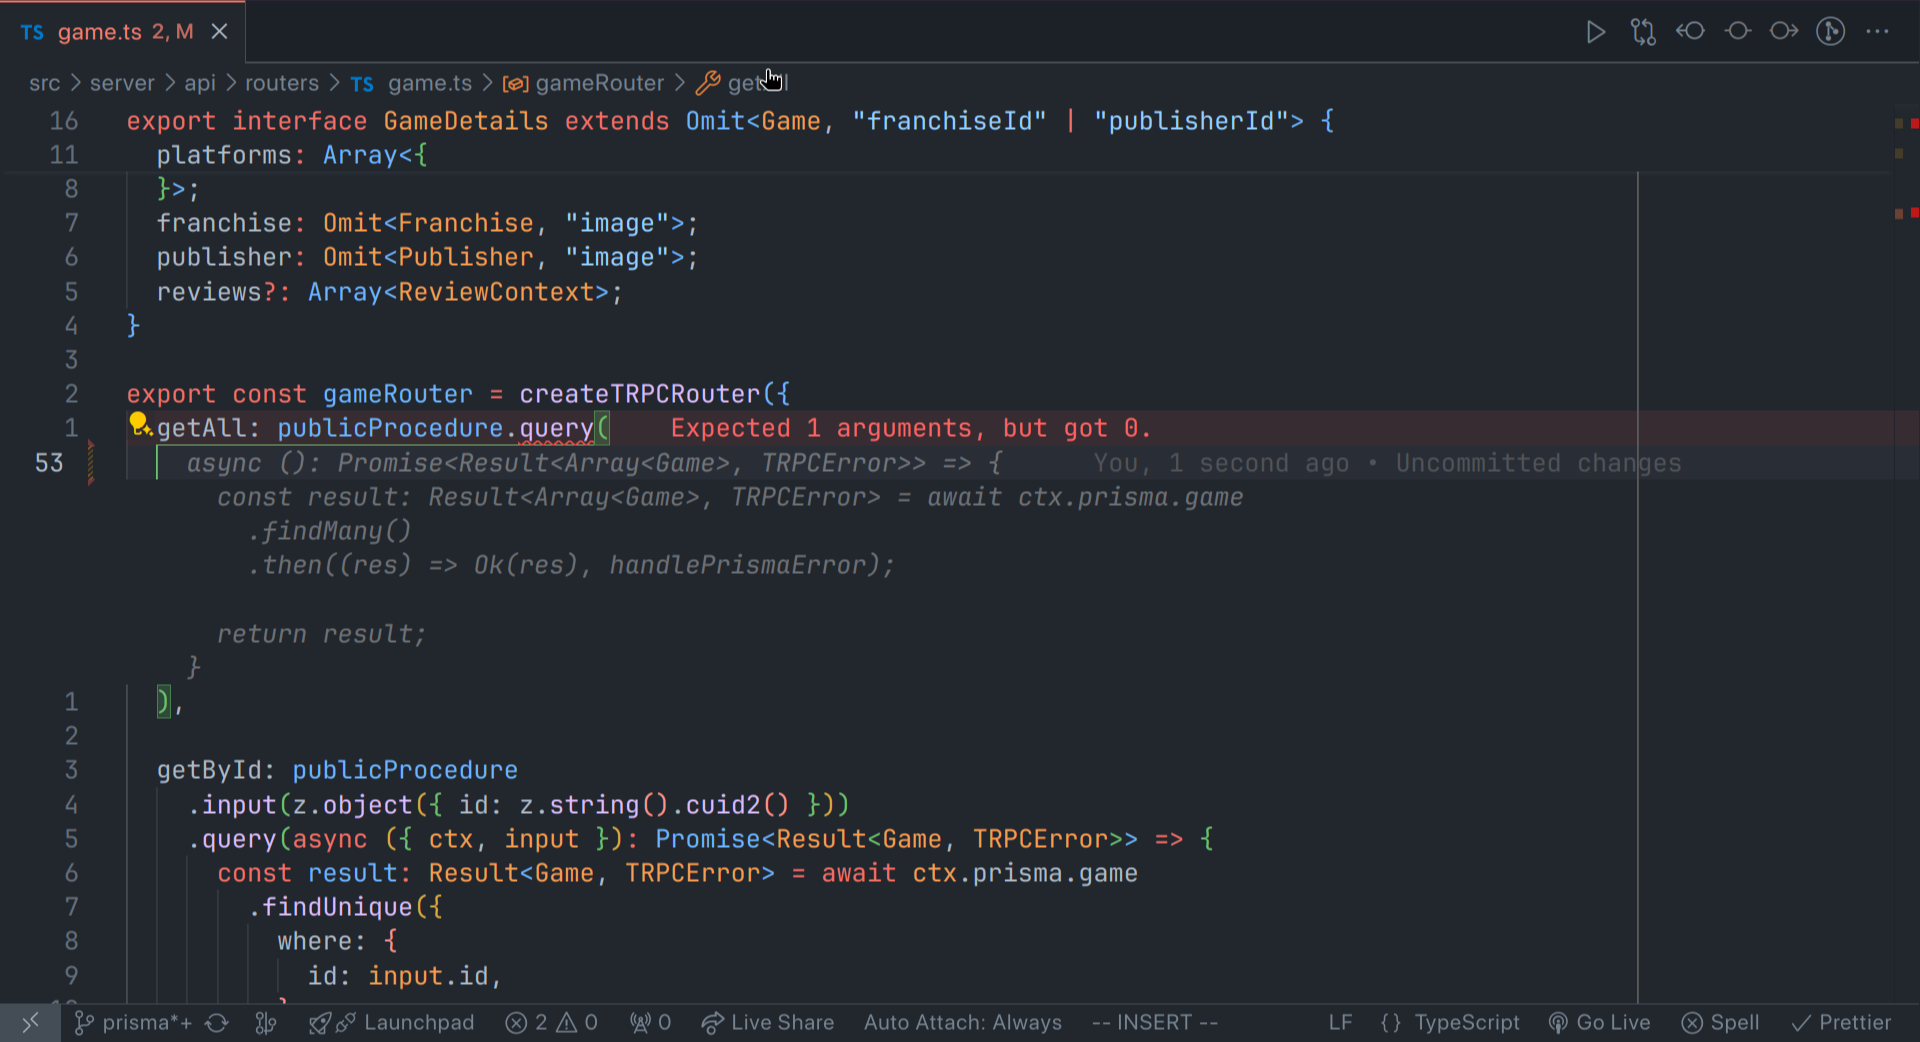
\includegraphics[width=\textwidth]{copilot.png}
    \label{fig:codeGen}
    \caption{Παράδειγμα Δημιουργίας Κώδικα σε πραγματικό χρόνo
      \textlatin{(real time code generation)} εντός του \textlatin{IDE}
      \textlatin{Visual Studio Code} από το \textlatin{GitHub Copilot }
    }
  \end{center}
\end{figure}

H παραγωγή κώδικα γίνεται με διάφορους βαθμούς λεπτομέρειας. Αρχικά, το
μοντέλο υπολογίζει το επόμενο σύμβολο του κώδικα χρησιμοποιώντας
\textlatin{\textbf{next token prediction}} \cite{Izadi2022,Kim2021,Wang2021,Feng2020,Ciniselli2021b,Ciniselli2021a}.
Στο στάδιο της ολοκλήρωσης ολόκληρης σειράς κώδικα, το μοντέλο
χρησιμοποιεί ένα κομμάτι συγκείμενου κώδικα.
\cite{Izadi2022,Guo2022,Svyatkovskiy2020,Lu2021}. Στο μέγιστο δυνατό
βαθμό, το μοντέλο μπορεί να παράγει ολόκληρες συναρτήσεις ή κλάσεις.
\cite{fried2023incoder,Guo2022,githubcopilot}.

Η παραγωγή κώδικα επίσης μπορεί να λάβει υπ' όψιν αποκλειστικά το
συγκείμενο κώδικα πριν την θέση του κέρσορα στο αρχείο ή και τον κώδικα
που ακολουθεί την θέση του κέρσορα. \cite{izadi2024language} Το μοντέλο
του \textlatin{GitHub Copilot} χρησιμοποιεί την δεύτερη προσέγγιση,
παράγοντας κώδικα που συμπληρώνει τον υπάρχοντα κώδικα του
προγραμματιστή. \cite{githubcopilot,fried2023incoder, wang2021codet5}.
Κατά την έρευνα λήφθηκε η απόφαση να χρησιμοποιηθεί, ως επί το πλείστον,
η λειτουργία \textlatin{GitHub Copilot Chat} για την έρευνα και τα
πειράματα, κυρίως γιατί ο σύγκειμενος κώδικας που χρησιμοποιεί το
μοντέλο κατά την λειτουργία αύτη, μπορεί να επιλεχθεί είτε από το
μοντέλο, είτε συγκεκριμένα από τον προγραμματιστή. Ένας ακόμα λόγος που
επιλέχθηκε η χηση του \textlatin{GitHub Copilot Chat}, είναι ότι η
καταγραφή του κώδικα που παράχθηκε κατά την έρευνα από το μοντέλο ήταν
πολύ δυσκολότερηη με την χρήση του \textlatin{GitHub Copilot}, καθώς η
δημιουργία κώδικα σε πραγματικό χρόνο \textlatin{(\textbf{real time code
    generation})} ήταν πολύ δύσκολη αυτής του \textlatin{GitHub Copilot
  Chat}.

\begin{figure}[H]
  \begin{center}
    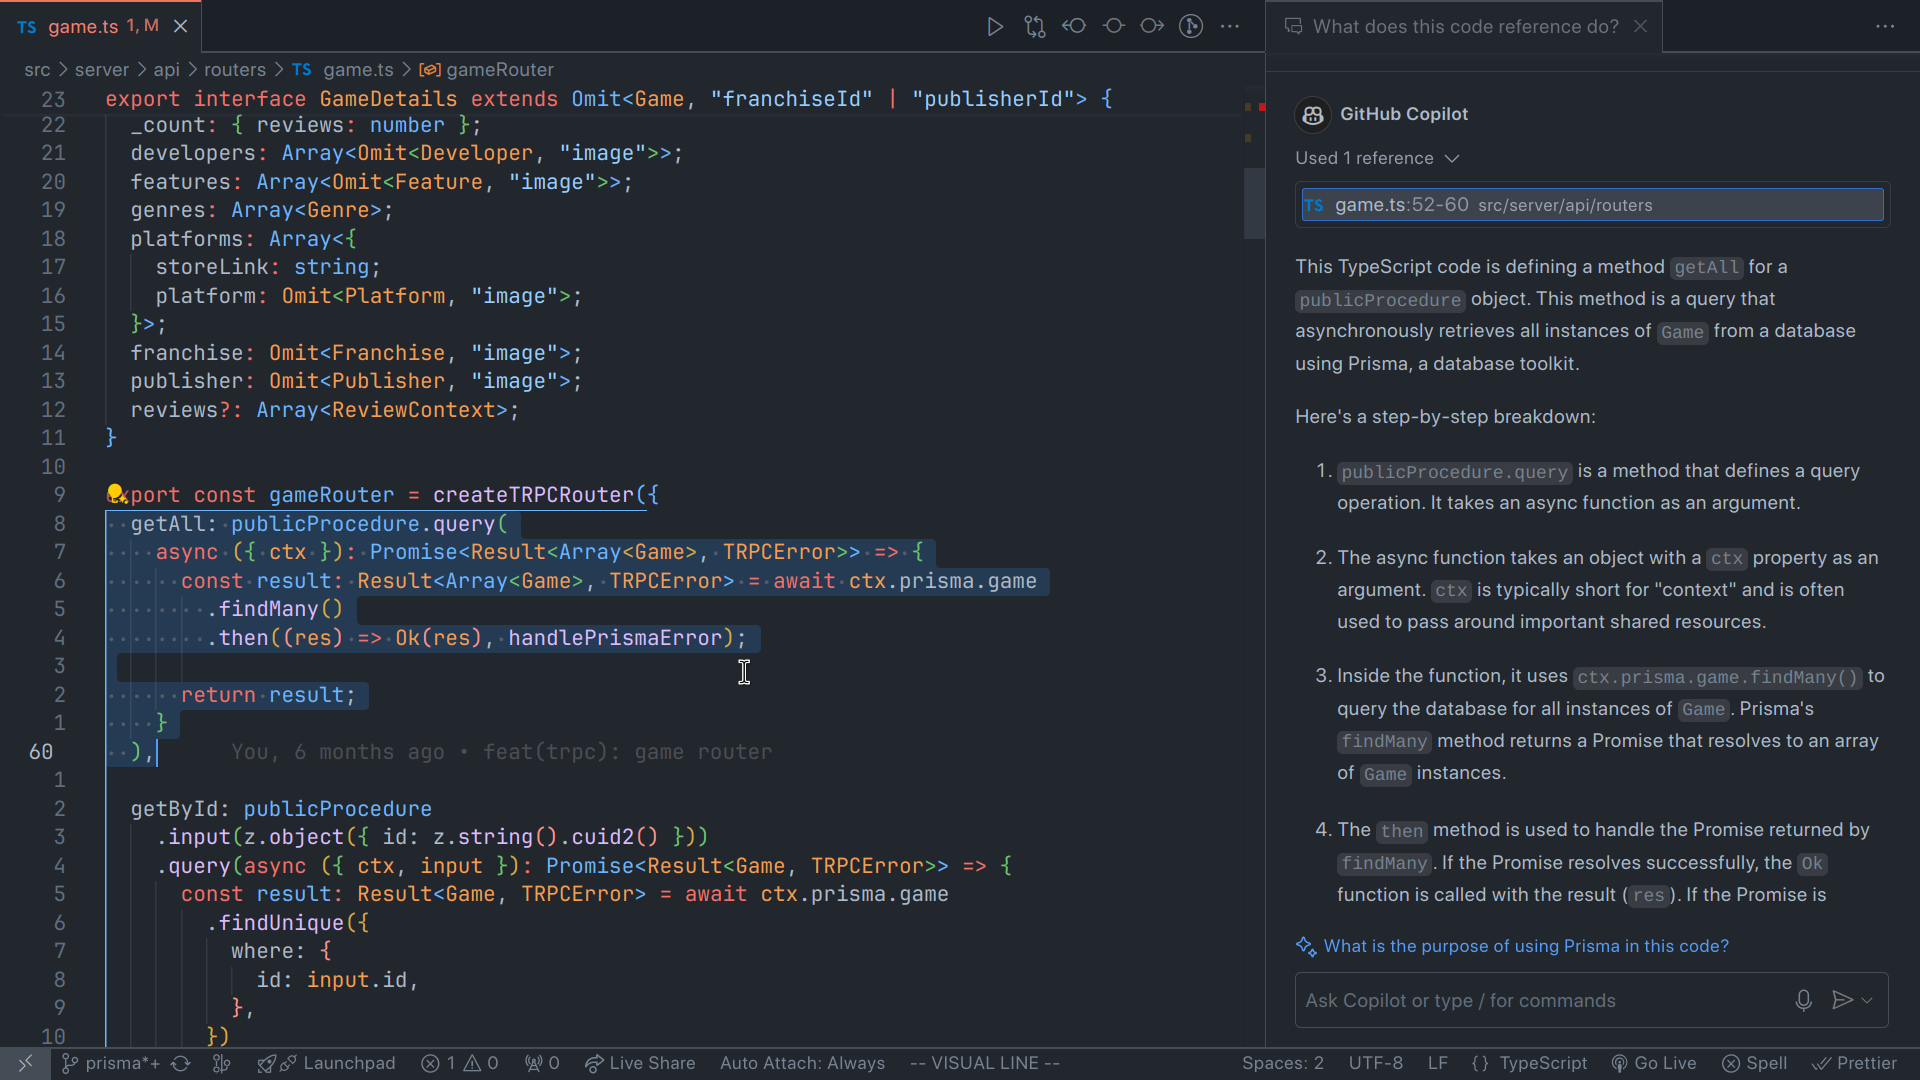
\includegraphics[width=\textwidth]{reference.png}
    \label{fig:reference}
    \caption{Παράδειγμα Δημιουργίας Κώδικα σε πραγματικό χρόνo
      \textlatin{(real time code generation)} εντός του \textlatin{IDE}
      \textlatin{Visual Studio Code} από το \textlatin{GitHub Copilot }
    }
  \end{center}
\end{figure}
